%% 学位论文入口，填写扉页与答辩信息并引入各篇章。


%% =================================================================
%% 1. 文档类设置（请根据个人实际情况选择对应的文档类参数）
%% =================================================================
%% 学术学位博士（与官方模板示例一致）：
\documentclass[phd,phil]{buptthesis}

%% 其它学位类型（取消相应注释即可使用）：
%% \documentclass[master,phil]{buptthesis}   % 学术学位硕士
%% \documentclass[master,eng]{buptthesis}    % 专业学位硕士
%% \documentclass[phd,eng]{buptthesis}       % 专业学位博士

%% 选项说明：
%% master / phd : 硕士学位 / 博士学位，默认 master
%% phil / eng   : 学术学位 / 专业学位，默认 phil
%% blind        : 盲审版（扉页作者/学号/导师匿名，答辩委员会置空，并自动排除致谢）

%% =================================================================
%% 2. 用户宏包与自定义配置（可选）
%% =================================================================
% 在此加载论文专用宏包。

%% =================================================================
%% 3. 论文元数据填写（请按实际情况填写）
%% =================================================================

%% 中文扉页信息
\BUPTthesiscntitlepage{%
  confidential = {公开},                  % 密级：仅限涉密学生改写，默认“公开”
  title = {标题\\标题},                    % 论文题目（不超过36个汉字，超长自动折行加下划线）
  studentid = {0000000000},               % 10位学号
  name = {张三},                           % 作者姓名
  major = {学科专业},                      % 学科专业（一级/二级学科或专业学位领域）
  trainingmode = {学习方式},               % 培养方式：全日制 / 非全日制
  supervisor = {李四},                     % 导师姓名（可写“李四”“李四 教授”等形式）
  institute = {学院}                       % 所在学院
}

%% 日期配置
\BUPTdateOptions{%
  pageYear = {2026},                     % 扉页年份
  pageMonth = {10},                      % 扉页月份
  pageDay = {31},                        % 扉页日期
  dissertationYear = {},                 % 答辩年份（送审版本可留空）
  dissertationMonth = {},                % 答辩月份
  dissertationDay = {}                   % 答辩日期
}

%% 英文扉页信息（英文扉页无密级行，与官方模板一致）
\BUPTthesisentitlepage{%
  titleEN = {Title\\Title},
  studentidEN = {0000000000},
  nameEN = {Zhang San},
  majorEN = {Subject},
  supervisorEN = {Li Si},
  instituteEN = {Institute}
}

%% 答辩委员会名单（送审前版本可留空；答辩后终版如实填写）
\BUPTdissertationcommitteepage{%
  chairName = {},
  chairTitle = {},
  chairOrgan = {},
  memberAName = {},
  memberATitle = {},
  memberAOrgan = {},
  memberBName = {},
  memberBTitle = {},
  memberBOrgan = {},
  memberCName = {},
  memberCTitle = {},
  memberCOrgan = {},
  memberDName = {},
  memberDTitle = {},
  memberDOrgan = {},
  secretaryName = {},
  secretaryTitle = {},
  secretaryOrgan = {}
}

%% 独创性声明扫描替换页（可选：如果已有签字盖章的整页扫描版PDF，取消下行注释指定文件路径即可）
%% \statementpage{figures/signed_statement.pdf}

%% =================================================================
%% 4. 论文正文排版架构
%% =================================================================
\begin{document}

%% ---------------- 扉页与版权声明部分 ----------------
\makechinesetitle      % 中文扉页
\makeenglishtitle      % 英文扉页
\makecommitteelist     % 答辩委员会名单
\makestatement         % 独创性声明与论文使用授权说明

%% ---------------- 前言部分（大写罗马数字页码） ----------------
\frontmatter
%% 中文摘要示例内容。


\begin{cnabstract}
文本文本文本文本文本文本文本文本文本文本文本文本文本文本文本文本文本文本文本文本文本文本文本文本文本文本文本文本文本文本文本文本文本文本文本文本文本文本文本文本文本文本文本文本文本文本文本文本文本文本文本文本文本文本文本。

文本文本文本文本文本文本文本文本文本文本文本文本文本文本文本文本文本文本文本文本文本文本文本文本文本文本文本文本文本文本文本文本文本文本文本文本文本文本文本文本。文本文本文本文本文本文本文本文本文本文本文本文本文本文本文本文本文本文本文本文本文本文本文本文本文本文本文本文本文本文本文本文本文本文本文本文本文本文本文本文本。

\cnkeywords{关键词1；关键词2；关键词3；关键词4}
\end{cnabstract}
      % 中文摘要及关键词
%% 英文摘要示例内容。


\begin{enabstract}
Text text text text text text text text text text text text text text text, text text text text text text text, text text text text text text text text text text text text text text. Text text text text text text text text text text text text text text text, text text text text text text text, text text text text text text text text text text text text text text. Text text text text text text text text text text text text text text text, text text text text text text text, text text text text text text text text text text text text text text. Text text text text text text text text text text text text text text text, text text text text text text text, text text text text text text text text text text text text text text. Text text text text text text text text text text text text text text text, text text text text text text text, text text text text text text text text text text text text text text.

Second paragraph text text text text text text text text text text text text text text, text text text text text text text, text text text text text text text text text text text text text text. Text text text text text text text text text text text text text text text, text text text text text. Second paragraph text text text text text text text text text text text text text text, text text text text text text text, text text text text text text text text text text text text text text. Text text text text text text text text text text text text text text text, text text text text text.
\enkeywords{keyword1; keyword2; keyword3; keyword4}
\end{enabstract}
      % 英文摘要及关键词
\tableofcontents
%% 符号说明示例内容。


\begin{nomenclature}
  \begin{nomenclaturetable}{*{3}{B{104.15bp}}}
    符\quad 号 & 代表意义 & 单\quad 位 \\
    \textit{A}       & 截面积；散热面积 & m\textsuperscript{2} \\
    \textit{F}       & 力               & N \\
    \textit{e}       & 电子电荷         & C \\
    \textit{I, i}    & 电流             & A \\
    \textit{m}       & 质量             & kg \\
    \textit{Q}       & 热量       & kJ \\
    \textit{H}       & 比焓             & kJ/kg \\
    \textit{S}       & 比熵             & kJ/(kg·K) \\
  \end{nomenclaturetable}
\end{nomenclature}
    % 符号说明（三列表格）

%% ---------------- 正文部分（阿拉伯数字页码，从第1页重新编排） ----------------
\mainmatter
%% 第一章 绪论示例内容。


\chapter{绪论}

正文文字正文文字正文文字正文文字正文文字正文文字正文文字正文文字正文文字正文文字正文文正文文字正文文字正文文字正文文字正文文字正文文字正文文字正文文字。

\section{标题}

正文文字正文文字正文文字正文文字正文文字正文文字正文文字正文文字正文文正文文字正文文字正文文字正文文字正文文字正文文字正文文字正文文字正文文字正文文字正文文字正文文字。

正文文字正文文字正文文字正文文字正文文字正文文字正文文字正文文字正文文正文文字正文文字正文文字正文文字正文文字正文文字。

正文文字正文文字正文文字正文文字正文文字正文文字正文文字正文文字正文文正文文字正文文字正文文字正文文字正文文字正文文字\footnote{脚注文本脚注文本脚注文本脚注文本}。

正文文字正文文字正文文字正文文字正文文字正文文字正文文字正文文字正文文字正文文字正文文字正文文正文文字正文文字正文文字正文文字正文文字正文文字。

%% 三线表、表注和数据来源示例。


\begin{table}[!ht]
  \caption{表名}
  \label{tab:table11}
  \begin{thesistabular}{B{92.8bp}B{124.5bp}B{83.1bp}B{42.3bp}B{42.7bp}}
    \toprule
    XXXX & XXXX & XXXX & XXXX & XXXX \\
    \midrule
    XXXX & XXXX & XXXX & XXXX & XXXX \\
    XXXX & XXXX & XXXX & XXXX & XXXX \\
    XXXX & XXXX & XXXX & XXXX & XXXX \\
    XXXX & XXXX & XXXX & XXXX & XXXX \\
    XXXX & XXXX & XXXX & XXXX & XXXX \\
    XXXX & XXXX & XXXX & XXXX & XXXX \\
    \thesisbottomrule
  \end{thesistabular}
  \tablenote{注：如有需要可对表格进行注释说明，可省略。}
  \tablenote{数据来源：如需对数据来源进行说明，请参照此格式，可省略。}
\end{table}



正文文字正文文字正文文字正文文字正文文字正文文字正文文字正文文字正文文字正文文字正文文字正文文字正文文字正文文字正文文字文字文字文字文字文字文字文字文字文字文字文字文字文字文字文字文字文字文字文字文字。

\subsection{标题}

正文文字正文文字正文文字正文文字正文文字正文文字正文文字正文文字正文文字正文文字正文文字正文文字正文文字正文文字正文文字正文文字正文文字正文文字正文文字正文文字正文文字正文文字正文文字正文文字。
\begin{thesisequation}
  \frac{dx}{dt} = K(1-x)
  \label{eq:example}
\end{thesisequation}

正文文字正文文字正文文字正文文字正文文字正文文字正文文字正文文字正文文字正文文字正文文字正文文字正文文字正文文字正文文字正文文字正文文字正文文字正文文字正文文字正文文字正文文字正文文字正文文字。

\begin{thesisfigure}
  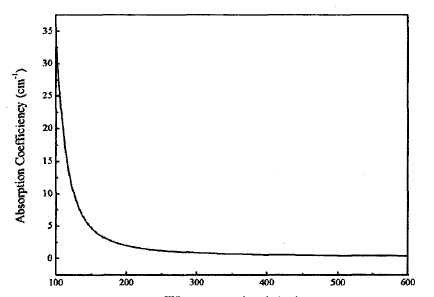
\includegraphics[width=251.6bp]{figures/chapter_01/figure_01.png}
  \caption{图名}
  \label{fig:figure11}
  \fignote{注：如有需要可对图片进行注释说明，可省略。}
  \fignote{图片来源：如需对图片来源进行说明，请参照此格式，可省略。}
\end{thesisfigure}

正文文字正文文字正文文字正文文字正文文字正文文字正文文字正文文字正文文字正文文字正文文字正文文字正文文字正文文字正文文字正文文字正文文字正文文字正文文字正文文字正文文字正文文字正文文字正文文字。

正文文字正文文字正文文字正文文字正文文字正文文字正文文字正文文字正文文字正文文字正文文字正文文字正文文字正文文字正文文字正文文字正文文字正文文字正文文字正文文字正文文字正文文字正文文字正文文字正文文字正文文字正文文字正文文字正文文字正文文字正文文字正文文字正文文字正文文字正文文字正文文字正文文字。

正文文字正文文字正文文字正文文字正文文字正文文字正文文字正文文字正文文字正文文字正文文字正文文字正文文字正文文字正文文字正文文字正文文字正文文字正文文字正文文字正文文字正文文字正文文字正文文字正文文字正文文字正文文字正文文字正文文字正文文字正文文字正文文字正文文字正文文字正文文字正文文字正文文字正文文字正文文字正文文字正文文字正文文字正文文字正文文字正文文字正文文字正文文字正文文字正文文字正文文字正文文字正文文字正文文字正文文字正文文字正文文字正文文字正文文字正文文字正文文字正文文字正文文字\cite{caoling2011}正文文字。

\begin{thesisfigure}
  \begin{subfigure}[b]{238.7bp}
    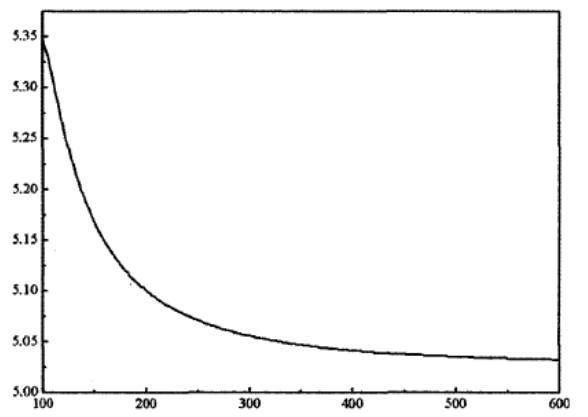
\includegraphics[width=\linewidth,height=168.25bp]{figures/chapter_01/figure_02_a.png}
    \caption{分图1}
  \end{subfigure}

  \begin{subfigure}[b]{233.8bp}
    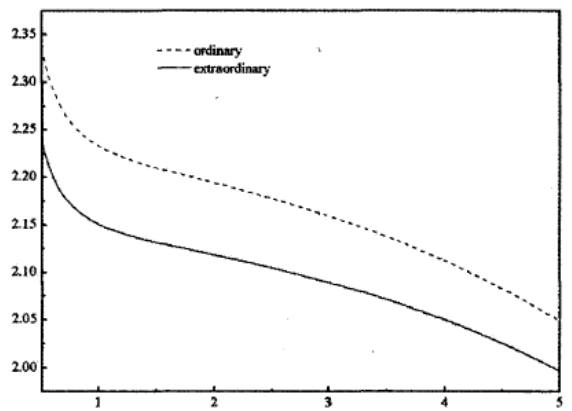
\includegraphics[width=\linewidth,height=168.25bp]{figures/chapter_01/figure_02_b.png}
    \caption{分图2}
  \end{subfigure}
  \caption{图名}
  \label{fig:figure12}
\end{thesisfigure}

正文文字正文文字正文文字正文文字正文文字正文文字正文文字正文文字正文文字正文文字正文文字正文文字正文文字正文文字正文文字正文文字正文文字正文文字正文文字正文文字正文文字正文文字正文文字正文文字。

正文文字正文文字正文文字正文文字正文文字正文文字正文文字正文文字正文文字正文文字正文文字正文文字正文文字正文文字正文文字正文文字正文文字正文文字正文文字正文文字正文文字正文文字正文文字正文文字。文文字正文文字正文文字正文文字正文文字。

正文文字正文文字正文文字正文文字正文文字正文文字正文文字正文文字正文文字正文文字正文文字正文文字。

\subsection{标题}

正文文字正文文字正文文字正文文字正文文字正文文字正文文字正文文字正文文字正文文字正文文字正文文字正文文字正文文字正文文字正文文字正文文字正文文字正文文字正文文字正文文字正文文字正文文字正文文字正文文字正文文字正文文字正文文字正文文字正文文字正文文字正文文字正文文字正文文字正文文字正文文字正文文字正文文字。

\subsubsection{标题}

正文文字正文文字正文文字正文文字正文文字正文文字正文文字正文文字正文文字正文文字正文文字正文文字正文文字正文文字正文文字正文文字正文文字正文文字正文文字正文文字正文文字。

\subsubsection{标题}

正文文字正文文字正文文字正文文字正文文字正文文字正文文字正文文字正文文字正文文字正文文字正文文字正文文字正文文字正文文字正文文字正文文字正文文字正文文字正文文字正文文字。

\subsection{标题}

正文文字正文文字正文文字正文文字正文文字正文文字正文文字正文文字正文文字正文文字正文文字正文文字正文文字正文文字正文文字正文文字正文文字正文文字正文文字正文文字正文文字正文文字正文文字正文文字。

正文文字正文文字正文文字正文文字正文文字正文文字正文文字正文文字正文文字正文文字正文文字正文文字正文文字正文文字正文文字正文文字正文文字正文文字正文文字正文文字正文文字正文文字正文文字正文文字。

正文文字正文文字正文文字正文文字正文文字正文文字正文文字正文文字正文文字正文文字正文文字正文文字正文文字正文文字正文文字正文文字正文文字正文文字正文文字正文文字正文文字正文文字正文文字正文文字。

正文文字正文文字正文文字正文文字正文文字正文文字正文文字正文文字正文文字正文文字正文文字正文文字正文文字正文文字正文文字正文文字正文文字正文文字正文文字正文文字正文文字正文文字正文文字正文文字。

正文文字正文文字正文文字正文文字正文文字正文文字正文文字正文文字正文文字正文文字正文文字正文文字正文文字正文文字正文文字正文文字正文文字正文文字正文文字正文文字正文文字正文文字正文文字正文文字文字正文文字正文文字文字正文文字正文文字。

%% 跨页长表及重复表头示例。


\begin{longtable}{*{5}{B{65.95bp}}}
  \caption{表名}\label{tab:table12}\\
  \toprule
  XXXX & XXXX & XXXX & XXXX & XXXX \\
  \midrule
  \endfirsthead

  \continuedtablecaption{表名} \\
  \toprule
  XXXX & XXXX & XXXX & XXXX & XXXX \\
  \midrule
  \endhead

  \thesisbottomrule
  \endfoot

  \thesisbottomrule
  \endlastfoot

  XXXX & XXXX & XXXX & XXXX & XXXX \\
  XXXX & XXXX & XXXX & XXXX & XXXX \\
  XXXX & XXXX & XXXX & XXXX & XXXX \\
  XXXX & XXXX & XXXX & XXXX & XXXX \\
  XXXX & XXXX & XXXX & XXXX & XXXX \\
  XXXX & XXXX & XXXX & XXXX & XXXX \\
  XXXX & XXXX & XXXX & XXXX & XXXX \\
  XXXX & XXXX & XXXX & XXXX & XXXX \\
  XXXX & XXXX & XXXX & XXXX & XXXX \\
  XXXX & XXXX & XXXX & XXXX & XXXX \\
  XXXX & XXXX & XXXX & XXXX & XXXX \\
  XXXX & XXXX & XXXX & XXXX & XXXX \\
  XXXX & XXXX & XXXX & XXXX & XXXX \\
  XXXX & XXXX & XXXX & XXXX & XXXX \\
  XXXX & XXXX & XXXX & XXXX & XXXX \\
  XXXX & XXXX & XXXX & XXXX & XXXX \\
\end{longtable}



\section{标题}

正文文字正文文字正文文字正文文字正文文字正文文字正文文字正文文字正文文字正文文字正文文字正文文字正文文字正文文字正文文字正文文字正文文字正文文字正文文字正文文字正文文字正文文字正文文字正文文字。

\section{标题}

正文文字正文文字正文文字正文文字正文文字正文文字正文文字正文文字正文文字正文文字正文文字正文文字正文文字正文文字正文文字正文文字正文文字正文文字正文文字正文文字正文文字正文文字正文文字正文文字正文文字。
 % 第一章 绪论
%% 第二章 标题示例内容。


\chapter{标题}

正文文字正文文字正文文字正文文字正文文字正文文字正文文字正文文字正文文字正文文字正文文字正文文字正文文字正文文字正文文字正文文字正文文字正文文字正文文字正文文字正文文字正文文字正文文字正文文字。

\section{标题}

正文文字正文文字正文文字正文文字正文文字正文文字正文文字正文文字正文文字正文文字正文文字正文文字正文文字正文文字正文文字正文文字正文文字正文文字正文文字正文文字正文文字正文文字正文文字正文文字。

\subsection{标题}

正文文字正文文字正文文字正文文字正文文字正文文字正文文字正文文字正文文字正文文字正文文字正文文字正文文字正文文字正文文字正文文字正文文字正文文字正文文字正文文字正文文字正文文字正文文字正文文字。

正文文字正文文字正文文字正文文字正文文字正文文字正文文字正文文字正文文字正文文字正文文字正文文字正文文字正文文字正文文字正文文字正文文字正文文字正文文字正文文字正文文字正文文字正文文字正文文字。

正文文字正文文字正文文字正文文字正文文字正文文字正文文字正文文字正文文字正文文字正文文字正文文字正文文字正文文字正文文字正文文字正文文字正文文字正文文字正文文字正文文字正文文字正文文字正文文字。

 % 第二章 标题
%% 第三章 标题示例内容。


\chapter{标题}

正文文字正文文字正文文字正文文字正文文字正文文字正文文字正文文字正文文字正文文字正文文字正文文字正文文字正文文字正文文字正文文字正文文字正文文字正文文字正文文字正文文字正文文字正文文字正文文字。

\section{标题}

正文文字正文文字正文文字正文文字正文文字正文文字正文文字正文文字正文文字正文文字正文文字正文文字正文文字正文文字正文文字正文文字正文文字正文文字正文文字正文文字正文文字正文文字正文文字正文文字。

\subsection{标题}

正文文字正文文字正文文字正文文字正文文字正文文字正文文字正文文字正文文字正文文字正文文字正文文字正文文字正文文字正文文字正文文字正文文字正文文字正文文字正文文字正文文字正文文字正文文字正文文字。

正文文字正文文字正文文字正文文字正文文字正文文字正文文字正文文字正文文字正文文字正文文字正文文字正文文字正文文字正文文字正文文字正文文字正文文字正文文字正文文字正文文字正文文字正文文字正文文字正文文字正文文字正文文字正文文字。

正文文字正文文字正文文字正文文字正文文字正文文字正文文字正文文字正文文字正文文字正文文字正文文字正文文字正文文字正文文字正文文字正文文字正文文字正文文字正文文字正文文字正文文字正文文字正文文字正文文字正文文字正文文字正文文字正文文字正文文字正文文字正文文字正文文字正文文字正文文字正文文字。

 % 第三章 标题
%% 第四章 标题示例内容。


\chapter{标题}

正文文字正文文字正文文字正文文字正文文字正文文字正文文字正文文字正文文字正文文字正文文字正文文字正文文字正文文字正文文字正文文字正文文字正文文字正文文字正文文字正文文字正文文字正文文字正文文字。

\section{标题}

正文文字正文文字正文文字正文文字正文文字正文文字正文文字正文文字正文文字正文文字正文文字正文文字正文文字正文文字正文文字正文文字正文文字正文文字正文文字正文文字正文文字正文文字正文文字正文文字。

\subsection{标题}

正文文字正文文字正文文字正文文字正文文字正文文字正文文字正文文字正文文字正文文字正文文字正文文字正文文字正文文字正文文字正文文字正文文字正文文字正文文字正文文字正文文字正文文字正文文字正文文字。

正文文字正文文字正文文字正文文字正文文字正文文字正文文字正文文字正文文字正文文字正文文字正文文字正文文字正文文字正文文字正文文字正文文字正文文字正文文字正文文字正文文字正文文字正文文字正文文字。

正文文字正文文字正文文字正文文字正文文字正文文字正文文字正文文字正文文字正文文字正文文字正文文字正文文字正文文字正文文字正文文字正文文字正文文字正文文字正文文字正文文字正文文字正文文字正文文字。

 % 第四章 标题
%% 第五章 结论示例内容。


\chapter{结论}

正文文字正文文字正文文字正文文字正文文字正文文字正文文字正文文字正文文字正文文字正文文字正文文字正文文字正文文字正文文字正文文字正文文字正文文字正文文字正文文字正文文字正文文字正文文字正文文字。

正文文字正文文字正文文字正文文字正文文字正文文字正文文字正文文字正文文字正文文字正文文字正文文字正文文字正文文字正文文字正文文字正文文字正文文字正文文字正文文字正文文字正文文字正文文字正文文字。

 % 第五章 结论

%% ---------------- 参考文献部分（GB/T 7714-2015 格式） ----------------
%% 本示例展示多种文献类型。写作时删除下一行，文献表随正文引用生成。
\nocite{*}
\bibliographystyle{gbt7714-numerical}
\bibliography{main}

%% ---------------- 附录与后置章节 ----------------
%% 附录示例内容。


\begin{appendixpage}
正文文字正文文字正文文字正文文字正文文字正文文字正文文字正文文字正文文字正文文字正文文字正文文字正文文字正文文字正文文字正文文字正文文字正文文字正文文字正文文字正文文字正文文字正文文字正文文字。
\end{appendixpage}
        % 附录
\BUPTifblind{}{%% 致谢示例内容。


\begin{acknowledgement}
正文文字正文文字正文文字正文文字正文文字正文文字正文文字正文文字正文文字正文文字正文文字正文文字正文文字正文文字正文文字正文文字正文文字正文文字正文文字正文文字正文文字正文文字正文文字正文文字。

正文文字正文文字正文文字正文文字正文文字正文文字正文文字正文文字正文文字正文文字正文文字正文文字正文文字正文文字正文文字正文文字正文文字正文文字正文文字正文文字正文文字正文文字正文文字正文文字。
\end{acknowledgement}
} % 致谢
%% 攻读学位期间取得的创新成果目录示例内容。


\begin{publication}
% 写作时用实际条目替换下列占位段落，按成果取得时间排序。
% 例如：1. 成果题名，刊物名称，2026 年 1 月，第 10 卷第 1 期，第 1–10 页，署名第 1。
正文文字正文文字正文文字正文文字正文文字正文文字正文文字正文文字正文文字正文文字正文文字正文文字正文文字正文文字正文文字正文文字正文文字正文文字正文文字正文文字正文文字正文文字正文文字正文文字。

正文文字正文文字正文文字正文文字正文文字正文文字正文文字正文文字正文文字正文文字正文文字正文文字正文文字正文文字正文文字正文文字正文文字正文文字正文文字正文文字正文文字正文文字正文文字正文文字。
\end{publication}
     % 攻读学位期间取得的创新成果目录
%% 作者学习经历示例内容。


\begin{experience}
  \begin{experiencetable}[|E{108bp}|E{45.36bp}|E{137.52bp}|E{132.96bp}|]
    \hline
    起止年月 & 类别 & 学习单位名称 & 学科/专业名称 \\
    \hline
    & & & \\
    \hline
    & & & \\
    \hline
    & & & \\
    \hline
    & & & \\
    \hline
    & & & \\
    \hline
    & & & \\
    \hline
    & & & \\
    \hline
  \end{experiencetable}
\end{experience}
      % 作者学习经历

\end{document}
